%%%%%%%%%%%%%%%%%%%%%%%%%%%%%%%%%%%%%%%%%%%%%%%%%%%%%%%%%%%%%%%%%
\chapter{Financial Report}  \newpage
%%%%%%%%%%%%%%%%%%%%%%%%%%%%%%%%%%%%%%%%%%%%%%%%%%%%%%%%%%%%%%%%%

% FiscalReport.tex - STATIC report body. Edit this prose freely.
% All numbers and data tables come from % ILSA-commands.tex - GENERATED by treasurer.py. Do not edit by hand.
% Re-run: python src/treasurer.py --year YYYY   (or --start/--end)
% The report body (FiscalReport.tex) inserts these commands.

\newcommand{\ilsaBudgetFyLabel}{August 2025 -- July 2026}
\newcommand{\ilsaBudgetRows}{Aug & 370 & 241 & \$900 & \$783 & \$117 \\
Sep & 425 & 259 & \$1,000 & \$904 & \$96 \\
Oct & 490 & 295 & \$1,200 & \$1,011 & \$189 \\
Nov & 560 & 351 & \$1,350 & \$1,712 & -\$362 \\
Dec & 650 & 385 & \$1,580 & \$1,767 & -\$187 \\
Jan & 750 & 653 & \$1,800 & \$1,805 & -\$5 \\
Feb & 850 & 720 & \$2,100 & --- & --- \\
Mar & 980 & 728 & \$2,400 & \$2,214 & \$186 \\
Apr & 1,120 & 905 & \$2,750 & --- & --- \\
May & 1,300 & 957 & \$3,200 & --- & --- \\
Jun & 1,500 & 1,000 & \$3,650 & --- & --- \\
Jul & 1,700 & --- & \$4,200 & --- & --- \\}
\newcommand{\ilsaBudgetTotal}{\textbf{Total} & --- & --- & \textbf{\$26,130} & \textbf{\$10,196} & \\}
\newcommand{\ilsaCashflowYearRows}{Opening reserves & \$0 & \$26,700 & \$167,603 & \$0 \\
Total income & \$26,702 & \$149,046 & \$20,795 & \$196,543 \\
Total expenses & (\$1) & (\$8,144) & (\$4,519) & (\$12,664) \\
\textbf{Net change} & \textbf{\$26,700} & \textbf{\$140,902} & \textbf{\$16,276} & \textbf{\$183,879} \\
\textbf{Closing reserves} & \textbf{\$26,700} & \textbf{\$167,603} & \textbf{\$183,879} & \textbf{\$183,879} \\}
\newcommand{\ilsaExpenseYearRows}{Program -- Imagination Library & \$0 & \$8,144 & \$4,019 & \$12,163 \\
Other (fees, chargebacks) & \$1 & \$0 & \$500 & \$501 \\}
\newcommand{\ilsaExpenseYearTotal}{\textbf{Total expenses} & \textbf{\$1} & \textbf{\$8,144} & \textbf{\$4,519} & \textbf{\$12,664} \\}
\newcommand{\ilsaGrantCount}{11}
\newcommand{\ilsaGrantPct}{95.7\%}
\newcommand{\ilsaGrantTotal}{\$188,047}
\newcommand{\ilsaIncomeMonthly}{\$9,359}
\newcommand{\ilsaIncomeYearRows}{Recurring giving (PayPal + Bonterra) & \$1,502 & \$5,878 & \$1,116 & \$8,495 \\
Grants \& major gifts (bank deposits) & \$25,200 & \$143,168 & \$19,679 & \$188,047 \\}
\newcommand{\ilsaIncomeYearTotal}{\textbf{Total income} & \textbf{\$26,702} & \textbf{\$149,046} & \textbf{\$20,795} & \textbf{\$196,543} \\}
\newcommand{\ilsaLargestGift}{\$110,000}
\newcommand{\ilsaLargestGiftMonth}{December 2025}
\newcommand{\ilsaNMonths}{21}
\newcommand{\ilsaNetChange}{\$183,879}
\newcommand{\ilsaOpSentence}{did not fully cover this cost, leaving an operating deficit of \$3,668 that was funded from grants and accumulated reserves.}
\newcommand{\ilsaOpexRows}{Mail Box & \$350 & yearly &  \\}
\newcommand{\ilsaOtherTotal}{\$501}
\newcommand{\ilsaPeriod}{September 2024--May 2026}
\newcommand{\ilsaProgramCount}{12}
\newcommand{\ilsaProgramMonthly}{\$579}
\newcommand{\ilsaProgramSlope}{\$61}
\newcommand{\ilsaProgramTotal}{\$12,163}
\newcommand{\ilsaProjCashEnd}{\$80,193}
\newcommand{\ilsaProjCashEndOpt}{\$110,478}
\newcommand{\ilsaProjCashEndPess}{\$41,557}
\newcommand{\ilsaProjCashOneYr}{\$167,908}
\newcommand{\ilsaProjCashTwoYr}{\$141,847}
\newcommand{\ilsaProjEndOneYr}{May 2027}
\newcommand{\ilsaProjEndTwoYr}{May 2028}
\newcommand{\ilsaRecurringMonthly}{\$405}
\newcommand{\ilsaRecurringPct}{4.3\%}
\newcommand{\ilsaRecurringSlope}{-\$9}
\newcommand{\ilsaRecurringTotal}{\$8,495}
\newcommand{\ilsaReportTitle}{Fiscal Report}
\newcommand{\ilsaReservesEnd}{\$183,879}
\newcommand{\ilsaReservesStart}{\$0}
\newcommand{\ilsaScenBand}{15\%}
\newcommand{\ilsaScenEnd}{December 2029}
\newcommand{\ilsaScenReserveRows}{Dec 2026 & \$175,377 & \$175,789 & \$176,238 \\
Dec 2027 & \$149,641 & \$153,932 & \$158,126 \\
Dec 2028 & \$106,454 & \$121,984 & \$135,580 \\
Dec 2029 & \$41,557 & \$80,193 & \$110,478 \\}
\newcommand{\ilsaTotalExpense}{\$12,664}
\newcommand{\ilsaTotalIncome}{\$196,543}
\newcommand{\ilsaYearA}{2024}
\newcommand{\ilsaYearB}{2025}
\newcommand{\ilsaYearC}{2026}
 (generated by
% src/treasurer.py). Re-run treasurer.py to refresh the numbers; edit this file
% to change wording, structure, or styling.

\section{Financial Overview (\ilsaPeriod)}

\subsection{Executive Summary}

The Imagination Library of San Antonio (ILSA) is a 501(c)(3) nonprofit and Local
Program Partner of Dolly Parton's Imagination Library, mailing free books each
month to children from birth to age five in San Antonio. This report summarizes
financial activity over the \ilsaNMonths{} months of \ilsaPeriod{}.

During this period ILSA received \ilsaTotalIncome{} in total income against
\ilsaTotalExpense{} in expenses. Accumulated reserves stood at \ilsaReservesEnd{}
at the close of the period.

\begin{itemize}
    \item \textbf{Recurring giving} (online donations and subscriptions via PayPal
          and Bonterra): \ilsaRecurringTotal{} (\ilsaRecurringPct{} of income),
          averaging \ilsaRecurringMonthly{} per month.
    \item \textbf{Grants and major gifts} (deposited at the bank): \ilsaGrantTotal{}
          (\ilsaGrantPct{} of income) across \ilsaGrantCount{} deposits; the largest
          was \ilsaLargestGift{} in \ilsaLargestGiftMonth{}.
    \item \textbf{Program cost} (Imagination Library age-group, welcome, and
          graduation books plus per-piece mailing): \ilsaProgramAccrual{} invoiced,
          of which \ilsaProgramPaid{} has been paid in cash and
          \ilsaProgramPayable{} remains an outstanding payable to the Dollywood
          Foundation. Program cost averages \ilsaCostPerChild{} per child served.
\end{itemize}

Recurring giving \ilsaOpSentence{} This is the central dynamic of ILSA's finances:
day-to-day donations do not yet cover the cost of the book program, so the
organization relies on periodic grants and major gifts to build and sustain
reserves.

\subsection{Income}

\begin{table}[h]
\centering
\begin{tabular}{|l|r|r|r|r|}
\hline
\textbf{Income Source} & \textbf{\ilsaYearA} & \textbf{\ilsaYearB} & \textbf{\ilsaYearC} & \textbf{Total} \\
\hline
\ilsaIncomeYearRows
\hline
\ilsaIncomeYearTotal
\hline
\end{tabular}
\caption{Income by source and calendar year (2024 and 2026 are partial; data spans \ilsaPeriod{}).}
\end{table}

Recurring giving is the predictable, forecastable stream. Grants and major gifts
are episodic by nature and are reported as discrete events rather than a trend.

\subsection{Expenses}

\begin{table}[h]
\centering
\begin{tabular}{|l|r|r|r|r|}
\hline
\textbf{Expense Category} & \textbf{\ilsaYearA} & \textbf{\ilsaYearB} & \textbf{\ilsaYearC} & \textbf{Total} \\
\hline
\ilsaExpenseYearRows
\hline
\ilsaExpenseYearTotal
\hline
\end{tabular}
\caption{Operating expenses by calendar year, cash basis (Dollywood payments as cleared at the bank: \ilsaProgramCount{} payments over \ilsaPeriod{}). The invoiced (accrual) program cost is reconciled below.}
\end{table}

The program cost grows as enrollment increases, since ILSA pays per child served.
It is the organization's dominant and steadily rising expense.

\subsubsection*{Program Cost: Invoiced vs.\ Paid}

The Dollywood Foundation bills monthly for welcome, age-group, and graduation books
plus per-piece mailing. The \emph{invoiced} (accrual) amount is the cost incurred
that month; cash payments clear about a month later, so cumulative invoiced minus
paid is the outstanding payable. Reserves elsewhere in this report remain on the
cash basis, so they continue to tie to actual money on hand.

\begin{table}[h]
\centering
\begin{tabular}{|l|r|r|r|}
\hline
\textbf{Year} & \textbf{Invoiced (accrual)} & \textbf{Paid (cash)} & \textbf{Payable (cumulative)} \\
\hline
\ilsaProgramReconRows
\hline
\ilsaProgramReconTotal
\hline
\end{tabular}
\caption{Program cost invoiced vs.\ paid, by calendar year. ``Payable'' is the cumulative invoiced-minus-paid balance owed to the Dollywood Foundation.}
\end{table}

\subsection{Cash Flow and Reserves}

\begin{table}[h]
\centering
\begin{tabular}{|l|r|r|r|r|}
\hline
\textbf{Cash Flow Component} & \textbf{\ilsaYearA} & \textbf{\ilsaYearB} & \textbf{\ilsaYearC} & \textbf{Full Period} \\
\hline
\ilsaCashflowYearRows
\hline
\end{tabular}
\caption{Consolidated cash flow by calendar year. Reserves are inception-to-date, so each year's opening equals the prior year's closing. Internal PayPal--bank transfers are netted out so donations are counted once.}
\end{table}

Closing reserves of \ilsaReservesEnd{} are healthy, but it should be understood
that the bulk of these reserves originates from one-time grants and major gifts
rather than from recurring operations.

\subsection{Outlook}

Projections extend the period's linear trend of recurring giving and program cost
forward, holding grants at zero (new grants are not assumed). On that basis:

\begin{itemize}
    \item Recurring-giving trend: \ilsaRecurringSlope{} per month.
    \item Program-cost trend: \ilsaProgramSlope{} per month.
    \item Projected reserves: \ilsaProjCashOneYr{} by \ilsaProjEndOneYr{} and
          \ilsaProjCashTwoYr{} by \ilsaProjEndTwoYr{}.
\end{itemize}

Because grants are episodic and excluded from the projection, this is a
deliberately conservative view: a single new grant or major gift materially
improves the outlook. The practical implication is that sustaining and growing
\emph{recurring} giving is the key to long-term operating sustainability.

\section{Budget and Forward Plan}

\subsection{Annual Operating Budget (\ilsaBudgetFyLabel)}

The board adopted the following enrollment and program-cost budget for the fiscal
year. Actual kids are the children served each month (age-group $+$ welcome $+$
graduation books mailed), and actual program cost is the invoiced (accrual) amount
for that invoice month; months not yet invoiced are shown as ``---''.

\begin{table}[h]
\centering
\small
\begin{tabular}{|l|r|r|r|r|r|}
\hline
\textbf{Month} & \textbf{Budget Kids} & \textbf{Actual Kids} & \textbf{Budget Inv.} & \textbf{Actual Inv.} & \textbf{Variance} \\
\hline
\ilsaBudgetRows
\hline
\ilsaBudgetTotal
\hline
\end{tabular}
\caption{Monthly enrollment and program-cost budget vs.\ actual, \ilsaBudgetFyLabel{}.}
\end{table}

\subsubsection{Operational and Marketing Costs}

\begin{table}[h]
\centering
\begin{tabular}{|l|r|l|p{4.5cm}|}
\hline
\textbf{Item} & \textbf{Budgeted} & \textbf{Frequency} & \textbf{Notes} \\
\hline
\ilsaOpexRows
\hline
\end{tabular}
\caption{Budgeted operational and marketing costs.}
\end{table}

\subsection{Reserve Projection Scenarios (through \ilsaScenEnd{})}

Reserves are projected from the linear trend of recurring giving and program cost
on past data (the baseline shown in the income-and-expense projection). The
optimistic and pessimistic scenarios vary that baseline net cash flow by
$\pm$\ilsaScenBand{} per year, widening the range over time. No new grants are
assumed, so all three are conservative views.

\begin{table}[h]
\centering
\begin{tabular}{|l|r|r|r|}
\hline
\textbf{Year-end} & \textbf{Pessimistic ($-$\ilsaScenBand{}/yr)} & \textbf{Baseline} & \textbf{Optimistic ($+$\ilsaScenBand{}/yr)} \\
\hline
\ilsaScenReserveRows
\hline
\end{tabular}
\caption{Projected reserves at each year-end under the baseline and $\pm$\ilsaScenBand{}/yr scenarios.}
\end{table}

Under the baseline, reserves decline from \ilsaReservesEnd{} today to
\ilsaProjCashEnd{} by \ilsaScenEnd{} (\ilsaProjCashEndPess{} pessimistic,
\ilsaProjCashEndOpt{} optimistic). The decline is gradual because recurring
giving nearly offsets the current program cost; the gap widens only as the
program grows. A single new grant or major gift -- excluded here by design --
would materially extend the runway.

\subsection{Governance and Compliance}

ILSA maintains its IRS 501(c)(3) tax-exempt status, complies with Texas nonprofit
corporation requirements, and operates under the partnership guidelines of Dolly
Parton's Imagination Library. Financial activity is reviewed by the board, with
segregation of duties across financial processes.

\subsection{Figures}

The figures that follow summarize the period. ``Monthly Income and Expense
Analysis'' separates recurring operating activity (top) from episodic grants and
major gifts (bottom), since the latter are large enough to obscure the former on a
single scale. ``Accumulated Reserves'' traces the consolidated cash position over
time, with grant events annotated. ``Income and Expense Projections'' extends the
recurring-giving and program-cost trends forward, and ``Projected Reserves''
carries that same baseline trend to \ilsaScenEnd{} with an optimistic/pessimistic
band of $\pm$\ilsaScenBand{} per year. The final map, ``San Antonio
Areas Served by ILSA,'' gives geographic context to the program's reach.

\begin{figure}[h]
\centering

\includegraphics[width=0.8\textwidth]{ILSA-Income-Debit-Actual.png}
\caption{Monthly Income and Expense Analysis}
\label{fig:income-debit}
\end{figure}

\begin{figure}[h]
\centering

\includegraphics[width=0.8\textwidth]{ILSA-Cash-Flow-Actual.png}
\caption{Accumulated Reserves}
\label{fig:cash-flow}
\end{figure}

\begin{figure}[h]
\centering

\includegraphics[width=0.8\textwidth]{ILSA-Cash-Flow-Projections.png}
\caption{Projected Reserves to \ilsaScenEnd{}: Baseline (linear trend) with $\pm$\ilsaScenBand{}/yr Optimistic and Pessimistic Scenarios}
\label{fig:projections}
\end{figure}

\begin{figure}[h]
\centering

\includegraphics[width=0.8\textwidth]{ILSA-Income-Debit-Projections.png}
\caption{Income and Expense Projections}
\label{fig:income-projections}
\end{figure}

\begin{figure}[h]
\centering
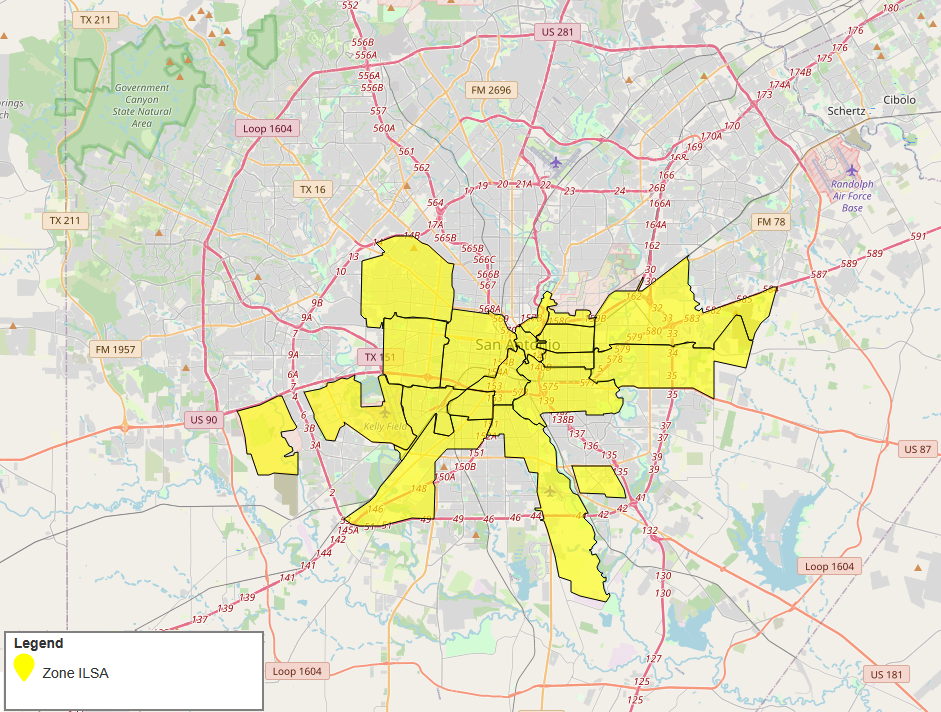
\includegraphics[width=0.8\textwidth]{Areas.png}
\caption{San Antonio Areas Served by ILSA}
\label{fig:areas}
\end{figure}

\vspace{1em}
\noindent\textit{Financial figures generated from ledger data by treasurer.py; see \texttt{ILSA-commands.tex}.}


%%%%%%%%%%%%%%%%%%%%%%%%%%%%%%%%%%%%%%%%%%%%%%%%%%%%%%%%%%%%%%%%%
% Enrollment cohorts and forward commitments (generated by src/cohort_explore.py
% via treasurer.py; figures in ../figures/cohort/, numbers in ILSA-commands.tex).
%%%%%%%%%%%%%%%%%%%%%%%%%%%%%%%%%%%%%%%%%%%%%%%%%%%%%%%%%%%%%%%%%
\section{Enrollment Cohorts and Forward Commitments}

Every enrolled child receives a book each month from birth through age five, so
the children on the rolls today are a multi-year financial commitment. This
section reads the invoice data as an age-structured population: each Imagination
Library Group~1--6 is a one-year age cohort; children age up one group per year
and graduate out after Group~6; new children enter through welcome books (invoice
item code \texttt{LETC}) and graduations are billed as \texttt{GRAD} books.
Tracking how these cohorts move through the system turns the current roster into a
forecast of future cost. Throughout, program cost is the invoiced
\ilsaCohortCostPerChild{} per child served (the accrual basis reconciled in the
Expenses section).

\subsection{Current Age Structure}

As of \ilsaCohortSnapshot{}, \ilsaCohortKids{} children are enrolled across the six
age groups (Figure~\ref{fig:cohort-pyramid}). The pyramid is \emph{inverted}: the
youngest group (Group~1, infants) is the smallest, while Groups~2--5 each hold
roughly two hundred children. This is the signature of a program still scaling up
by enrolling older children, rather than one fed primarily by newborns.

\begin{figure}[h]
\centering

\includegraphics[width=0.7\textwidth]{cohort/age_structure_snapshot.png}
\caption{Current enrollment by age group (the population pyramid that seeds the forward model).}
\label{fig:cohort-pyramid}
\end{figure}

The program has scaled rapidly --- from a handful of children in early 2025 to
over a thousand today --- and the stacked history (Figure~\ref{fig:cohort-history})
shows how each age group has filled in as enrollment has grown.

\begin{figure}[h]
\centering

\includegraphics[width=0.8\textwidth]{cohort/enrollment_by_group.png}
\caption{Monthly enrollment by age group since program launch, showing both total growth and the shifting age composition.}
\label{fig:cohort-history}
\end{figure}

\subsection{Observed Enrollment Flows}

The invoices now make the enrollment dynamics directly observable
(Figure~\ref{fig:cohort-flows}): welcome books (\texttt{LETC}) count new
enrollments each month, and graduation books (\texttt{GRAD}) count exits. New
enrollment averages about \ilsaCohortLetcAvg{} children per month with a linear
trend of \ilsaCohortLetcSlope{} per month. Two enrollment campaigns (December 2025
and March 2026) drive the visible spikes and pull that linear trend upward, so the
projection below should be read as an upper-leaning estimate of recruitment.

\begin{figure}[h]
\centering

\includegraphics[width=0.8\textwidth]{cohort/observed_flows.png}
\caption{Observed monthly enrollment inflow (\texttt{LETC}) versus graduation outflow (\texttt{GRAD}), with the linear recruitment trend used in the projection.}
\label{fig:cohort-flows}
\end{figure}

\subsection{Locked-in Commitment}

\begin{keyfinding}[Locked-in commitment]
Even if enrollment stopped today, the children already on the rolls obligate ILSA
to \ilsaCohortRunoffTotal{} of future books (\ilsaCohortBookMonths{} book-months) as
each cohort ages to graduation. This is the floor on program cost --- it assumes no
new enrollment and no attrition.
\end{keyfinding}

In headcount terms, the current cohort winds down from \ilsaCohortKids{} children
today to zero within six years as each group reaches graduation, with the oldest
groups (Group~6) leaving first and today's youngest children (Group~1) the last to
graduate (Figure~\ref{fig:cohort-runoff-kids}).

\begin{figure}[h]
\centering

\includegraphics[width=0.8\textwidth]{cohort/runoff_children.png}
\caption{Commitment runoff in children: today's enrolled population aged forward with no new enrollment, stacked by the group each child is in today.}
\label{fig:cohort-runoff-kids}
\end{figure}

The same runoff in dollars (Figure~\ref{fig:cohort-runoff}) gives the annual
committed cost and the cumulative remaining obligation.

\begin{figure}[h]
\centering

\includegraphics[width=0.8\textwidth]{cohort/runoff_dollars.png}
\caption{Commitment runoff for the current cohort with no new enrollment: annual committed cost and the cumulative remaining obligation.}
\label{fig:cohort-runoff}
\end{figure}

\subsection{Forward Projection to \ilsaCohortProjYear{}}

Carrying the observed recruitment trend forward, with graduation handled
endogenously (children age out at sixty months of enrollment), program cost
continues to climb (Figure~\ref{fig:cohort-cost}). Because the age at which new
children enter is not directly observed, two intake mixes bracket the outcome:
\emph{today's mix} (entrants skew older, as currently observed, so they graduate
sooner) and \emph{birth-fed} (a matured program enrolling mostly infants, who
carry a full six-year tail). The two diverge in age composition at the horizon
(Figure~\ref{fig:cohort-horizon}).

\begin{figure}[h]
\centering

\includegraphics[width=0.8\textwidth]{cohort/cost_projection.png}
\caption{Projected monthly program cost to \ilsaCohortProjYear{} under observed-\texttt{LETC} recruitment, with a $\pm$15\%/yr band and the two intake-mix scenarios.}
\label{fig:cohort-cost}
\end{figure}

By \ilsaCohortProjYear{}, enrollment reaches \ilsaCohortProjTodayKids{} children
(today's mix) to \ilsaCohortProjBirthKids{} (birth-fed), a monthly program cost of
\ilsaCohortProjTodayCost{} to \ilsaCohortProjBirthCost{}, and a locked-in future
commitment of \ilsaCohortProjTodayCommit{} to \ilsaCohortProjBirthCommit{}. The
intake mix is the dominant lever on the long-run liability.

\begin{keyfinding}[The intake age is the dominant lever]
By \ilsaCohortProjYear{}, monthly program cost reaches \ilsaCohortProjTodayCost{} to
\ilsaCohortProjBirthCost{}. The age at which new children enroll drives the long-run
liability: the locked-in commitment ranges from \ilsaCohortProjTodayCommit{}
(older-skew intake, as currently observed) to \ilsaCohortProjBirthCommit{}
(birth-fed, a matured program).
\end{keyfinding}

\begin{table}[h]
\centering
\small
\begin{tabular}{|l|r|r|r|r|}
\hline
\textbf{Year-end} & \textbf{Kids (today's)} & \textbf{Kids (birth-fed)} & \textbf{\$/mo (today's)} & \textbf{\$/mo (birth-fed)} \\
\hline
\ilsaCohortProjRows
\hline
\end{tabular}
\caption{Year-end enrollment and monthly program cost under the two intake-mix scenarios (``today's'' = current older-skew intake; ``birth-fed'' = matured program).}
\end{table}

\begin{figure}[h]
\centering

\includegraphics[width=0.7\textwidth]{cohort/horizon_pyramids.png}
\caption{Age structure at \ilsaCohortProjYear{} under each intake mix: birth-fed loads the young groups, producing a much larger long-run commitment tail.}
\label{fig:cohort-horizon}
\end{figure}